\section{Open-Meteo} \label{sec:openmeteo}
Open-Meteo is an open-source weather data platform and community-driven weather forecasting project. It aims to provide access to weather data and forecasts that are openly accessible to the public and can be used for a variety of applications, including research, development, and personal use.
It offers a diverse range of APIs that go
beyond traditional weather forecasting such as past weather data, ocean data, air quality, ensemble forecasts, climate forecasts based
on IPCC predictions, and even floods \cite{openmeteo}.
Open-Meteo offers over 80 years of hourly weather data, covering any location on earth, all at a 10 kilometer resolution. This extensive dataset is very useful to delve into the past and analyze historical weather patterns.

\begin{figure}[H]
	\centering
	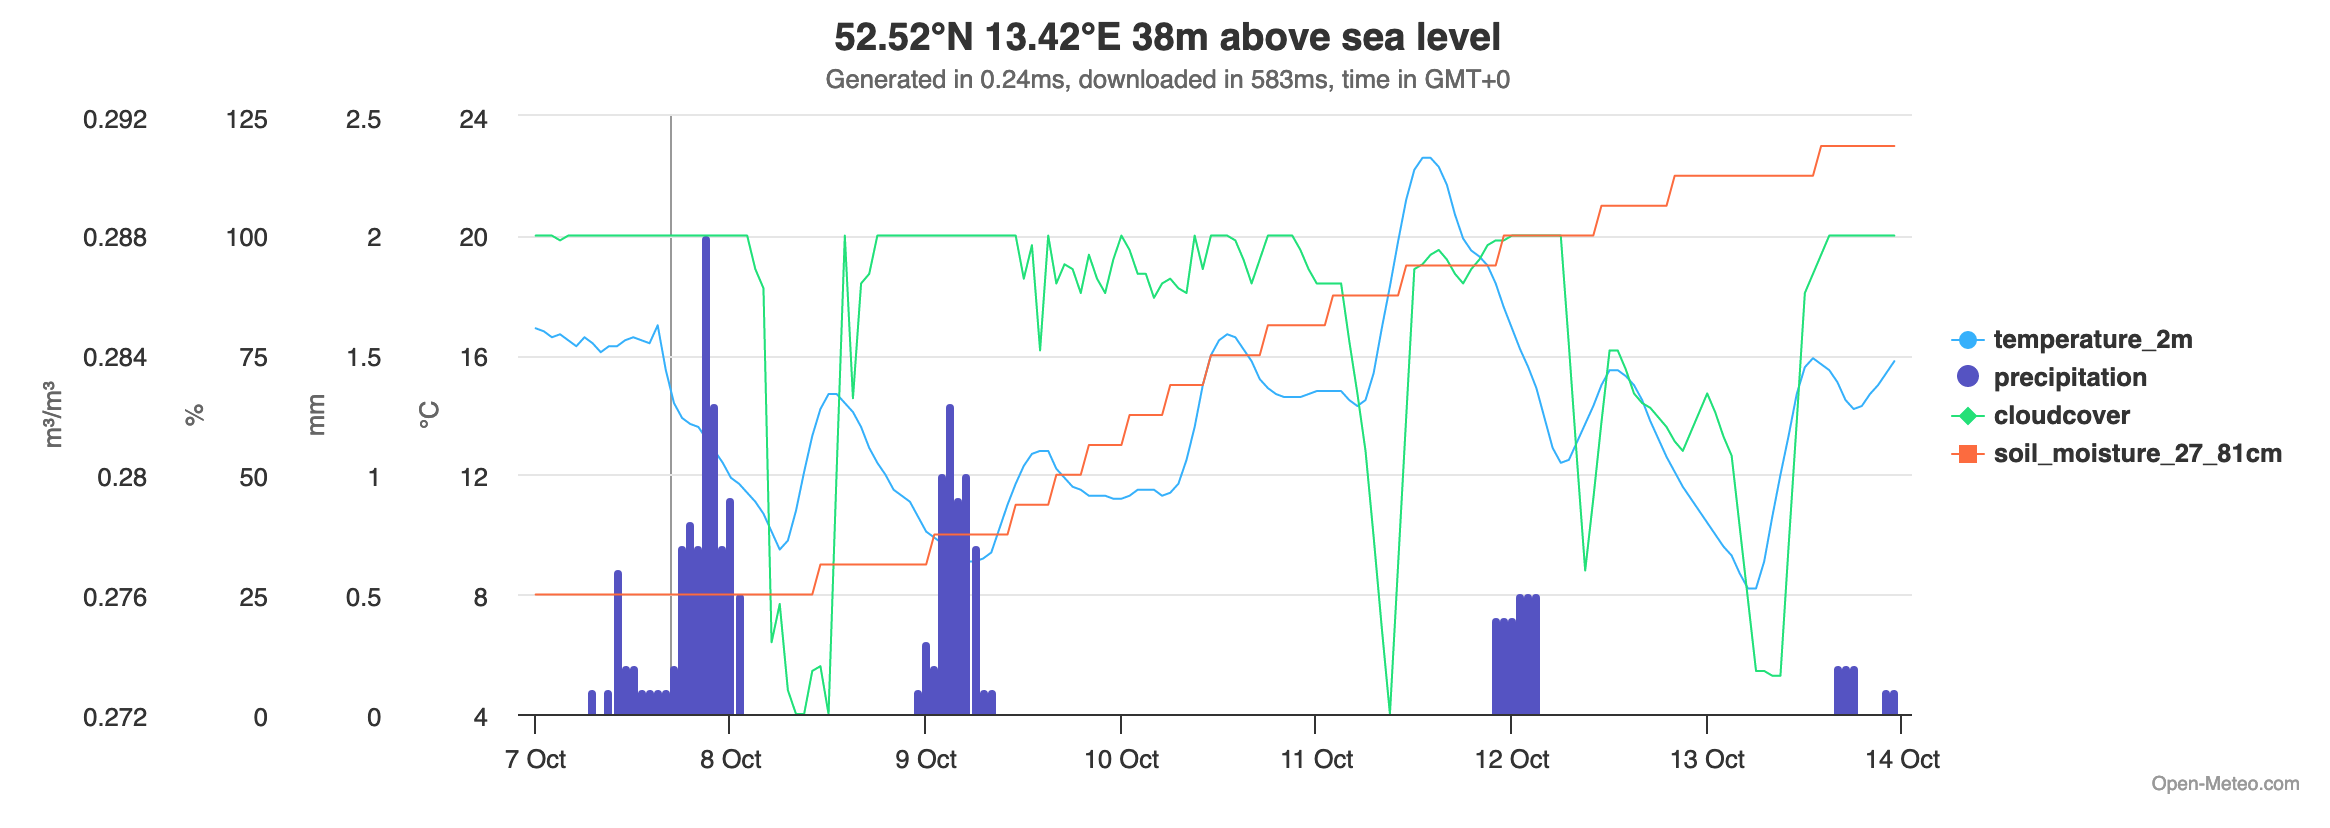
\includegraphics[width=\linewidth, keepaspectratio]{chapters/1_introduction/imgs/openmeteochart.png}
	\caption{A plot about some Open-Meteo data.}
	\label{fig:openmeteochart}
\end{figure}
\begin{figure}[H]
	\centering
	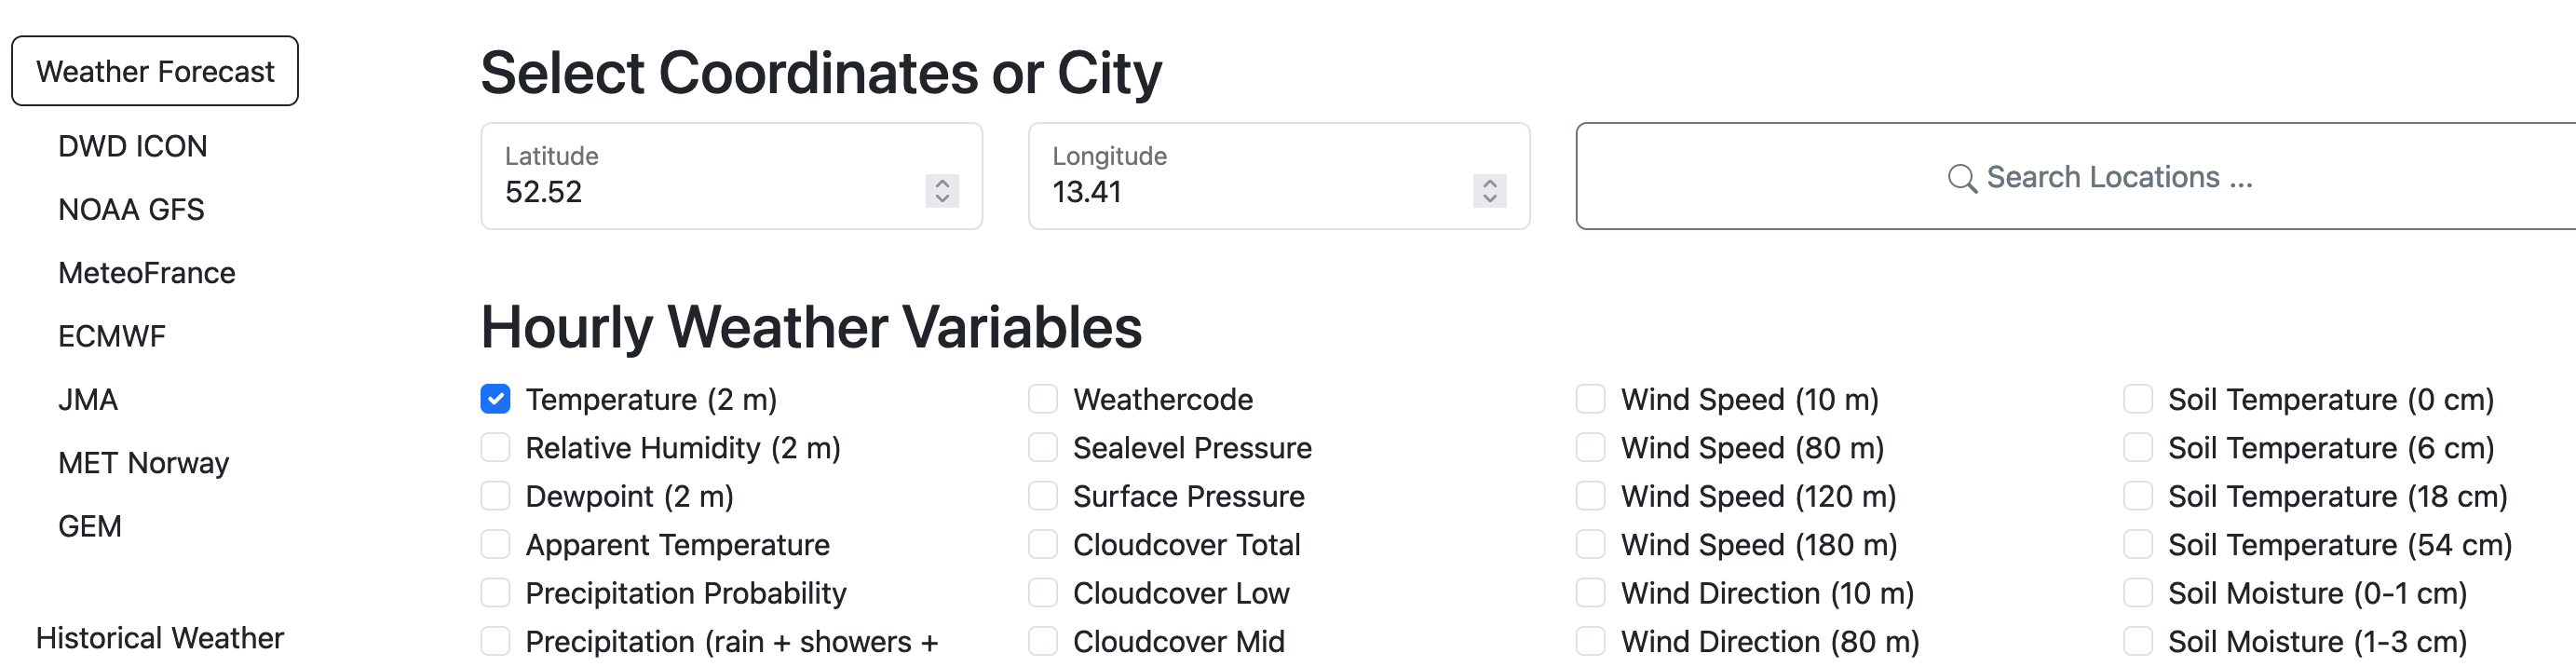
\includegraphics[width=\linewidth, keepaspectratio]{chapters/1_introduction/imgs/openmeteodata.png}
	\caption{Open-Meteo forecast features.}
	\label{fig:openmeteofetaures}
\end{figure}